% medgraph: addendum to the Phases 0-1 report, covering Phase 1e and Phase 2.
% Build: make report  (figures from scripts/report_figures.py, then latexmk -lualatex)
\documentclass[11pt,a4paper]{article}

\usepackage{fontspec}
\usepackage[a4paper,margin=2.4cm]{geometry}
\usepackage{microtype}
\usepackage{amsmath}
\usepackage{booktabs,tabularx,array,multirow}
\usepackage{graphicx}
\usepackage{xcolor}
\usepackage{tikz}
\usetikzlibrary{positioning,arrows.meta,fit,backgrounds,calc}
\usepackage{fancyvrb}
\usepackage{enumitem}
\usepackage[font=small,labelfont=bf]{caption}
\usepackage[hidelinks]{hyperref}

\definecolor{medblue}{HTML}{2a78d6}
\definecolor{medorange}{HTML}{eb6834}
\definecolor{muted}{HTML}{898781}
\definecolor{boxbg}{HTML}{f4f3ef}
\definecolor{boxline}{HTML}{c3c2b7}
\definecolor{kcond}{HTML}{c4462b}
\definecolor{kmed}{HTML}{2a78d6}
\definecolor{kproc}{HTML}{7a55c7}
\definecolor{kana}{HTML}{138a63}
\definecolor{krep}{HTML}{b7791f}
\definecolor{kenc}{HTML}{9aa3ad}

\newcommand{\code}[1]{\texttt{\detokenize{#1}}}
\setlist{itemsep=2pt,topsep=4pt}
\setlength{\emergencystretch}{2.5em}
\renewcommand{\arraystretch}{1.15}
\fvset{fontsize=\footnotesize,frame=single,rulecolor=\color{boxline},framesep=2mm}

\newenvironment{keybox}[1]
  {\par\smallskip\noindent\begin{tikzpicture}\node[draw=boxline,fill=boxbg,rounded corners=2pt,
   inner sep=6pt,text width=\dimexpr\linewidth-12pt\relax]\bgroup\textbf{#1}\par\smallskip}
  {\egroup;\end{tikzpicture}\par\smallskip}

\title{\textbf{medgraph}\\[6pt]
  \Large Addendum: Phases 1e and 2\\[4pt]
  \normalsize Hardened lab-report interpretation, checked on a fresh test set,\\
  and a per-patient knowledge graph with a timeline, a store and an offline viewer}
\author{enricotazzer}
\date{8 October 2026\\[2pt]\small Status: Phase~2 reviewed and approved; Phase~3 in progress}

\begin{document}
\maketitle

\begin{abstract}
\noindent This addendum continues the Phases~0--1 technical report (6 October 2026) and assumes it.

\textbf{Phase~1e} closed three of that report's open decisions before any report value could reach the patient graph.
\begin{itemize}[nosep]
  \item A \emph{row-order check} rejects a value copied from the reference range.
  \item The decimal separator and the order of day and month come from \emph{evidence in the report}, never from a guess. An ambiguous value or date is refused.
  \item Report rows carry the eGFR equation their printed name states.
\end{itemize}
The reports-v1 test split had been examined, so it became development data. A fresh, test-only set of 84 reports (reports-v2) was generated, with new patients and a new held-out layout, and run once with the prompt unchanged. On it, the LLM pipeline delivered every in-scope value printed under a known name (147 of 147, 95\% CI 97--100\%). It accepted no wrong value (0 of 150; the upper bound tightened from 6\% to 3\%) and stored no wrong date (0 of 84), in text and in PDF alike.

\textbf{Phase~2} turns each patient's record and filed lab reports into a typed graph.
\begin{itemize}[nosep]
  \item Every record becomes a node, and every edge states what it rests on: a reference in the data, time order, a value comparison, or a quoted guideline passage.
  \item A timeline holds only usable values, so everything else stays visible as a data note.
  \item Graphs are stored in SQLite with per-graph digests.
  \item An offline HTML viewer shows each patient.
\end{itemize}
All 1,148 synthetic patients were built with zero invariant violations. All 243 usable rows of the 156 filed reports repeat exactly one recorded FHIR value, which independently confirms that no wrong value or date got through extraction. Rebuilding with a different hash seed gives a byte-identical store digest.
\end{abstract}

\begin{keybox}{Scope and disclaimer}
All data in this report is synthetic: Synthea patients and template-generated lab reports. No real patient data and no MIMIC data was used or inspected. medgraph is a research prototype for decision support. It is not a medical device and does not diagnose; any clinical use would fall under the EU Medical Device Regulation. All numbers measure a software pipeline, not clinical performance.
\end{keybox}

\clearpage
\tableofcontents
\clearpage

%=====================================================================================
\section{Where this addendum starts}

The Phases~0--1 report ended with open decisions. Table~\ref{tab:open} shows what became of them. Items 1, 2 and 4 change what a report row \emph{is} when it reaches the graph: whether it is accepted, whether its date is certain, which equation it carries. They were therefore done first, as Phase~1e. Item~3 needs a screen where a person confirms each proposed name, so it moved to Phase~5.

\begin{table}[h]
\centering\small
\begin{tabularx}{\linewidth}{@{}l>{\raggedright\arraybackslash}X>{\raggedright\arraybackslash}p{4.4cm}@{}}
\toprule
\# & Open decision (Phases 0--1 report) & Outcome \\
\midrule
1 & Range-as-value guard & Phase 1e: row-order check, measured on a fresh set (Section~\ref{sec:order}) \\
2 & Ambiguity under an inferred locale & Phase 1e: conventions from evidence; ambiguous input refused (Section~\ref{sec:conv}) \\
3 & Unknown analyte names & Phase 5: the LLM proposes, a person confirms \\
4 & eGFR equation on report rows & Phase 1e: \code{ReportRow.method} \\
5 & Phase 2 and its persistence layer & SQLite and a local HTML viewer, both the user's choice (Section~\ref{sec:graph}) \\
\bottomrule
\end{tabularx}
\caption{The open decisions of the Phases~0--1 report.}
\label{tab:open}
\end{table}

\begin{table}[h]
\centering\small
\begin{tabularx}{\linewidth}{@{}lXl@{}}
\toprule
Phase & Scope & Status \\
\midrule
0 & Project setup, reproducible Synthea cohort, data profile & done \\
1 & FHIR ingestion, lab normalization, lab-report extraction and its evaluation (1a--1d); hardening (1e) & done \\
2 & Patient knowledge graph, timeline, store and viewer & done, approved \\
3 & Guideline rules and follow-up flags (KDIGO, WHO) & in progress \\
4 & Retrieval-augmented explanations; drug knowledge and medication-monitoring flags & planned \\
5 & Deployable application: API, frontend, containers & planned \\
6 & GNN research extension on MIMIC-IV (local models only) & planned \\
7 & Documentation and final results & planned \\
\bottomrule
\end{tabularx}
\caption{Project phases at the time of this addendum.}
\label{tab:phases}
\end{table}

%=====================================================================================
\section{Phase 1e: hardening report interpretation}

\subsection{The row-order check}
\label{sec:order}
The grounding check of Phase~1 rejects any transcribed field that does not occur in the report. It cannot see a \emph{genuine} string placed in the wrong field. On the reports-v1 test split, the model copied \texttt{< 200} from \texttt{214 mg/dL (rif. < 200)} as the value.

In every layout a result row reads name, value, unit, range. After grounding, \code{misplacement} therefore requires three things of the whitespace-squashed report text:
\begin{enumerate}[nosep]
  \item the value occurs after the analyte name, within 100 characters, with \textbf{no reference-range marker} in between: a label (\texttt{ref}, \texttt{rif}, \texttt{riferimento}, \texttt{reference}, \texttt{range}, \texttt{intervallo}), or a bracket opening onto a number or comparator (\texttt{(4,0}, \texttt{[< 200});
  \item a non-empty unit follows the value within 60 characters;
  \item a non-empty range follows that, within another 60.
\end{enumerate}
A row that fails gets the new status \code{misplaced}. It is kept for review and never used. The check runs before name mapping, so out-of-scope rows are checked too.

\subsection{Conventions from evidence, never guessed}
\label{sec:conv}
Phase~1 inferred en-GB or en-US from SI units, and the decimal separator from the language. On the synthetic data both were right by construction; on real reports a wrong guess swaps day and month, or reads \texttt{1.200} as 1.2.

\begin{itemize}
  \item \textbf{Decimal separator} (\code{decimal_separator_evidence}). Only a number with one separator followed by 1, 2 or 4+ digits proves which character is decimal (\texttt{13,5}, \texttt{0.70}). Three digits prove nothing. Dates, and clock times after a time word (\texttt{ore 08.30}), are skipped. Without proof, \texttt{1.200} is refused as ambiguous; every other value reads the same under both conventions. Proof that contradicts the language, or both separators in one report, becomes a report issue.
  \item \textbf{Date order} (\code{date_order_evidence}). Only a date with one field above 12 proves the order. A date with equal fields proves nothing about other dates. Italian reports are day-first by convention, and evidence still overrides it.
  \item \textbf{An ambiguous English date with no evidence is refused} (the user's decision). The report then has no collection date, and its rows stay off the timeline until a person confirms one. A date whose own digits settle it (\texttt{19/02/2024}) is always read.
\end{itemize}

\subsection{eGFR equation, and new metrics}
Report rows now carry \code{method}, taken from the printed name: \texttt{MDRD}, \texttt{CKD-EPI 2021}, \texttt{CKD-EPI (year not stated)} or \texttt{unspecified}. A name that states no equation is not assumed to use one.

The evaluation gained six metrics:
\begin{itemize}[nosep]
  \item misplaced rows;
  \item values refused as ambiguous;
  \item collection date \emph{not stored} and \emph{wrong}, which replace locale accuracy;
  \item language detection;
  \item decimal separator wrong;
  \item date order wrong.
\end{itemize}
The safety numbers are now two: wrong values accepted, and wrong dates.

\subsection{Re-scoring reports-v1, now development data}
Re-scoring needs no LLM calls, because the cached transcriptions are interpreted again by the current code.
\begin{itemize}
  \item \textbf{Row order.} The check rejected exactly the two range-as-value rows, and no correct row: none of the LLM's 186 development rows or 404 test rows, in text or PDF. All value metrics were unchanged.
  \item \textbf{Dates.} No date was stored wrongly. No date was stored for 4 of 24 development reports and 7 of 48 test reports: English reports whose dates all have both fields at most 12. Phase~1 had read them correctly, but only because its guess matched how the generator works.
  \item \textbf{A bug caught by the new metric.} The first version counted a date with equal fields (\texttt{09/09/2024}) as proof of day-first. Two en-US reports then had their collection date swapped. ``Collection date wrong'' exposed it; equal fields now prove nothing, and a test pins the case.
\end{itemize}

\subsection{A fresh test set: reports-v2}
reports-v1, including its test split, shaped these checks. Its test split had therefore become development data, and any new number needed a fresh set. reports-v2 (digest \texttt{dda930bb\ldots}) is designed as follows:
\begin{itemize}[nosep]
  \item \textbf{size:} 84 test-only reports, 6 per (layout family, language) cell, as text and PDF;
  \item \textbf{patients:} none of reports-v1's, excluded through the patient tags in its headers; reports-v1 itself regenerates unchanged;
  \item \textbf{layouts:} one new held-out family, \texttt{vertical} (one labelled field per line); only it counts as unseen;
  \item \textbf{names:} held-out names at a rate of 0.25 (0.5 before), which gives more accepted rows and so a tighter bound on wrong values;
  \item \textbf{content:} 619 rows per format, of which 147 are in scope under known names, and 26 in-scope rows have a one-sided range;
  \item \textbf{pipeline:} prompt \texttt{transcribe-v3}, unchanged since Phase~1; run once.
\end{itemize}

\begin{table}[h]
\centering\footnotesize
\begin{tabular}{@{}lrrr@{}}
\toprule
reports-v2 (84 reports, 619 rows) & LLM, text & LLM, PDF & rules, text \\
\midrule
\textbf{end-to-end, seen names} & \textbf{147/147} (97--100$^*$) & 147/147 & 56.5\% (43--69) \\
end-to-end, all in-scope rows & 74.6\% (68--81) & 74.6\% (68--81) & \\
row recall, unseen \texttt{vertical} layout & 100\% & 100\% & 0\% \\
\textbf{wrong values accepted} & \textbf{0 of 150} (0--3$^*$) & 0 of 150 & 0 of 84 (0--5$^*$) \\
rows rejected as misplaced & 0 of 619 (0--1$^*$) & 0 of 618 & 0 \\
\textbf{collection date wrong} & \textbf{0 of 84} (0--5$^*$) & 0 of 84 & 0 of 84 \\
collection date refused (not stored) & 7 of 84 & 7 of 84 & 7 of 84 \\
decimal separator / date order wrong & 0 / 0 & 0 / 0 & 0 / 0 \\
\bottomrule
\end{tabular}
\caption{reports-v2 results. Intervals: bootstrap over reports, or exact binomial ($^*$) at 0\% or 100\%.}
\label{tab:r2}
\end{table}

\begin{figure}[h]
\centering
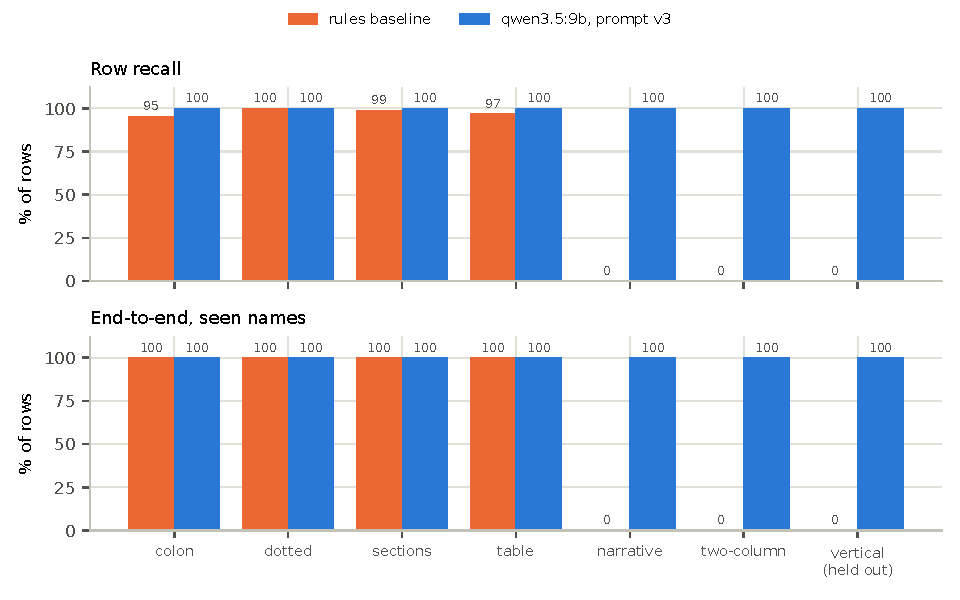
\includegraphics[width=0.92\linewidth]{figures/extraction-r2-by-family.pdf}
\caption{reports-v2 by layout family (text). Every family is test data here; only \texttt{vertical} was never seen in development. The narrative and two-column layouts were held out in reports-v1 but have since been examined, so they are no longer marked. The rules read none of the three layouts they were not written for.}
\label{fig:r2}
\end{figure}

\paragraph{Reading the results.}
\begin{itemize}
  \item \textbf{Safety held on fresh data.} No wrong value and no wrong date was accepted, in text or PDF, and the bound on wrong values tightened to 3\%.
  \item \textbf{No false rejections.} The row-order check rejected none of the 619 rows, including every row of the unseen layout.
  \item \textbf{The catch rate is not measured on fresh data.} The model never copied a range as a value on reports-v2: all 18 in-scope rows with a one-sided range under a known name were correct. Evidence that the check \emph{catches} the error remains the two reports-v1 rows and the unit tests.
  \item \textbf{The overall figure rose} from 59\% to 74.6\% because held-out names were rarer (0.25 instead of 0.5), not because the name table improved. Held-out names still mapped only 3 of 54, through the parenthetical rule.
  \item \textbf{Remaining transcription errors} (text): 43 units copied into the value, which code splits off, so end-to-end on known names stays at 100\%; five flag or range slips; in PDF, one missed row.
  \item \textbf{A weakness of grounding:} a one-character flag such as \texttt{H} occurs somewhere in almost every report, so grounding barely constrains it. The model returned \texttt{H} for a printed \texttt{alto} and the row was accepted. Flags never feed rules; values and dates do.
  \item \textbf{Cost:} median 62\,s per report (maximum 185\,s); 168 transcriptions took about 3\,h.
\end{itemize}

%=====================================================================================
\section{Phase 2: the patient graph}
\label{sec:graph}

\subsection{Decisions and design}
The user chose SQLite for persistence and a local HTML viewer. The design follows three facts about dev-1000:
\begin{itemize}
  \item \textbf{Records per patient:} the median patient has about 380 records and the largest about 19,000.
  \item \textbf{Stated reasons:} FHIR \code{reasonReference} names a condition on 77\% of medication requests and 27\% of procedures.
  \item \textbf{Reports print converted, rounded values:} creatinine recorded as 1.2345\,mg/dL may be printed as \texttt{109 µmol/L}.
\end{itemize}

Each patient is one \code{networkx.MultiDiGraph}, with deterministic node IDs (\code{<kind>:<source id>}) and edge kinds as edge keys. Attributes are the JSON form of pydantic models. Values travel as decimal strings with their digits, so a stored graph loads back identical. Figure~\ref{fig:schema} shows the schema.

\begin{figure}[h]
\centering
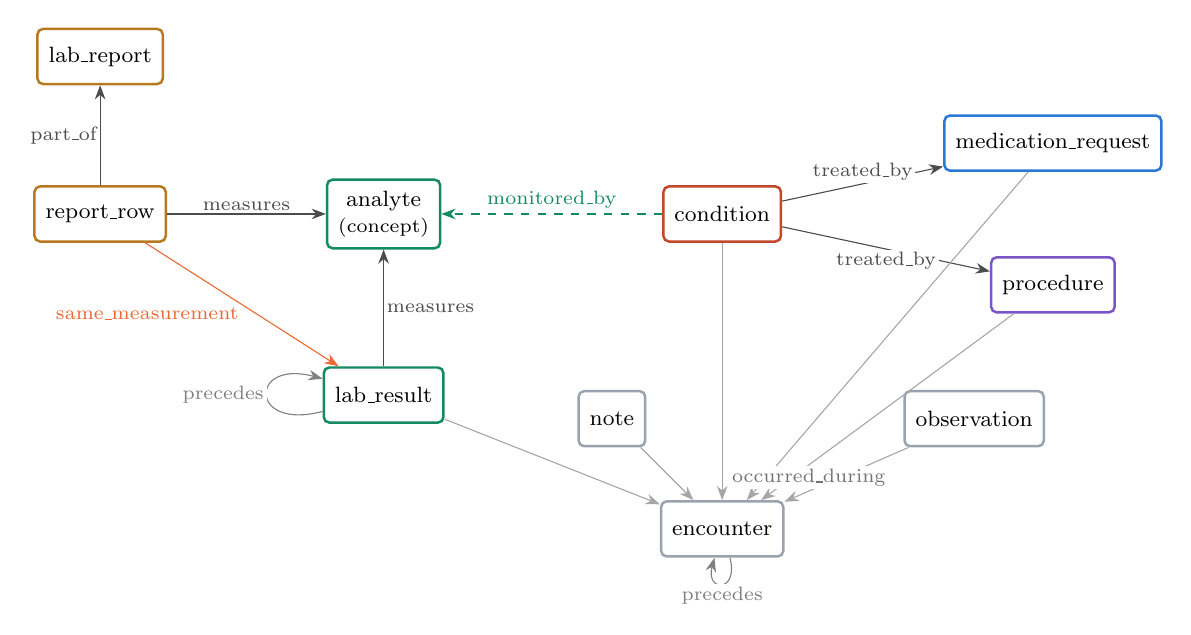
\begin{tikzpicture}[
  font=\footnotesize,
  kind/.style={draw=#1,line width=0.9pt,fill=white,rounded corners=2pt,inner sep=4pt,minimum height=0.7cm,align=center},
  e/.style={-{Stealth[length=1.8mm]},color=black!70},
  lbl/.style={font=\scriptsize,fill=white,inner sep=1pt}]
  \node[kind=kcond] (cond) at (0,0) {condition};
  \node[kind=kmed] (med) at (4.2,0.9) {medication\_request};
  \node[kind=kproc] (proc) at (4.2,-0.9) {procedure};
  \node[kind=kana] (ana) at (-4.3,0) {analyte\\\scriptsize(concept)};
  \node[kind=kana] (lab) at (-4.3,-2.3) {lab\_result};
  \node[kind=krep] (row) at (-7.9,0) {report\_row};
  \node[kind=krep] (rep) at (-7.9,2.0) {lab\_report};
  \node[kind=kenc] (enc) at (0,-4.0) {encounter};
  \node[kind=kenc] (obs) at (3.2,-2.6) {observation};
  \node[kind=kenc] (note) at (-1.4,-2.6) {note};
  \draw[e] (cond) -- node[lbl,above]{treated\_by} (med);
  \draw[e] (cond) -- node[lbl,below]{treated\_by} (proc);
  \draw[e,dashed,color=kana] (cond) -- node[lbl,above=1pt]{monitored\_by} (ana);
  \draw[e] (lab) -- node[lbl,right]{measures} (ana);
  \draw[e] (row) -- node[lbl,above]{measures} (ana);
  \draw[e] (row) -- node[lbl,left]{part\_of} (rep);
  \draw[e,color=medorange] (row) -- node[lbl,below left]{same\_measurement} (lab);
  \foreach \n in {cond,med,proc,lab,obs,note} \draw[e,color=black!35] (\n) -- (enc);
  \node[lbl,text=black!55] at (1.1,-3.35) {occurred\_during};
  \draw[e,color=black!50] (enc) edge[loop below,looseness=6] node[lbl,below]{precedes} (enc);
  \draw[e,color=black!50] (lab) edge[loop left,looseness=6] node[lbl,left]{precedes} (lab);
\end{tikzpicture}
\caption{Node and edge kinds (\code{graph/schema.py}). Every edge records its basis: a reference in the record (grey and black), a cited guideline passage (dashed green), a value comparison (orange) or time order. \code{precedes} also links consecutive report rows that are series points.}
\label{fig:schema}
\end{figure}

\paragraph{Usable values.} A measurement (lab result or report row) is \emph{usable} only with status \code{ok} and a date, and only usable values join a series. Everything else stays a node with the reason, for review: rejected, unmapped or implausible rows, unknown units, and rows of a report whose date was refused.

\paragraph{Guideline links.} \code{monitored_by} edges come from a small table in \code{rules/monitoring.py}. Each entry quotes its source verbatim, and the quotes were checked against the guideline text (Table~\ref{tab:monitor}). Codes are matched exactly, because medgraph has no SNOMED CT hierarchy. End-stage renal disease, renal transplant and diabetic kidney disease are deliberately left unlinked; Phase~3 decides them with its own citations. How often a test is due is also a Phase~3 rule. Phase~2 raises no flag.

\begin{table}[h]
\centering\footnotesize
\begin{tabularx}{\linewidth}{@{}>{\raggedright\arraybackslash}p{2.6cm}>{\raggedright\arraybackslash}p{2.4cm}>{\raggedright\arraybackslash}X@{}}
\toprule
Condition & Analytes & Source and quote \\
\midrule
CKD stages 1--4 & eGFR, urine ACR & KDIGO 2024, Practice Point 2.1.1 (executive summary, Kidney Int 2024;105:684--701): ``Assess albuminuria in adults, or albuminuria/proteinuria in children, and GFR at least annually in people with CKD.'' Practice Point 1.3.1.1 lists urine ACR first among albuminuria tests. \\
CKD stages 1--4 & creatinine & KDIGO 2024, Practice Point 1.2.2.1: ``Use serum creatinine (SCr) and an estimating equation for initial assessment of GFR.'' \\
Anaemia & haemoglobin & WHO 2024, Guideline on haemoglobin cutoffs (ISBN 978-92-4-008854-2), stated objective: ``\ldots the use of haemoglobin concentrations to assess anaemia''. \\
\bottomrule
\end{tabularx}
\caption{Cited condition-to-analyte links.}
\label{tab:monitor}
\end{table}

\paragraph{The same measurement in two sources.} Synthetic reports print FHIR values, converted and rounded, so a report row and a FHIR result can be one measurement. A report row with printed value $p$, which has $e$ digits after the decimal point, in a unit with canonical factor $f$, repeats a FHIR value with canonical value $v$ when
\[
\left|\, \frac{v}{f} - p \,\right| \;\le\; \tfrac12 \cdot 10^{-e},
\]
that is, when the recorded value, converted to the printed unit, rounds to what was printed. The analyte, the day and the comparator must also agree, and any eGFR equation the report names must be compatible with the LOINC code. For example, \texttt{109 µmol/L} repeats 1.2345\,mg/dL, which is 109.13\,µmol/L. A repeating row is not a second point: it corroborates the FHIR point, which then cites both sources. The approved plan had said ``equal canonical values''; that would almost never match a converted, rounded value, so this rule replaced it.

\paragraph{Timeline.} The timeline is read off the graph alone. It has three parts:
\begin{itemize}[nosep]
  \item \textbf{series} of usable values, each point with its sources;
  \item \textbf{events}: conditions, medications, procedures and encounters;
  \item \textbf{data notes}: single-value series, values set aside and why, undated reports, rejected and unmapped rows, rows counted once.
\end{itemize}
The notes state facts about the data; whether they matter clinically is for the rules.

\paragraph{Store.} One SQLite file per cohort, with tables \code{graphs}, \code{nodes}, \code{edges} and \code{meta}.
\begin{itemize}[nosep]
  \item Each patient's graph is replaced in a single transaction.
  \item Foreign keys refuse an edge without its nodes.
  \item Each graph's SHA-256 digest is stored and checked on load, which catches a tampered or corrupted row.
  \item A store written under another schema version is refused.
\end{itemize}

\paragraph{Viewer.} \code{make view} writes one self-contained page per patient (Figure~\ref{fig:viewer}).
\begin{itemize}[nosep]
  \item \textbf{Graph:} concepts, meaning records grouped by code. By default they sit in columns, left to right: lab reports, analytes, conditions, medications, procedures. A concept opens its records, and a record opens its values, sources and links.
  \item \textbf{Timeline:} event lanes, and one chart per lab series, with zoom kept in sync.
  \item \textbf{Libraries:} Cytoscape.js 3.34.3 and uPlot 1.6.32 are inlined, and their hashes are pinned in code and checked before rendering.
  \item \textbf{Offline and safe:} a Content Security Policy forbids every network request, and record text is written only with \code{textContent}.
\end{itemize}

\begin{figure}[h]
\centering
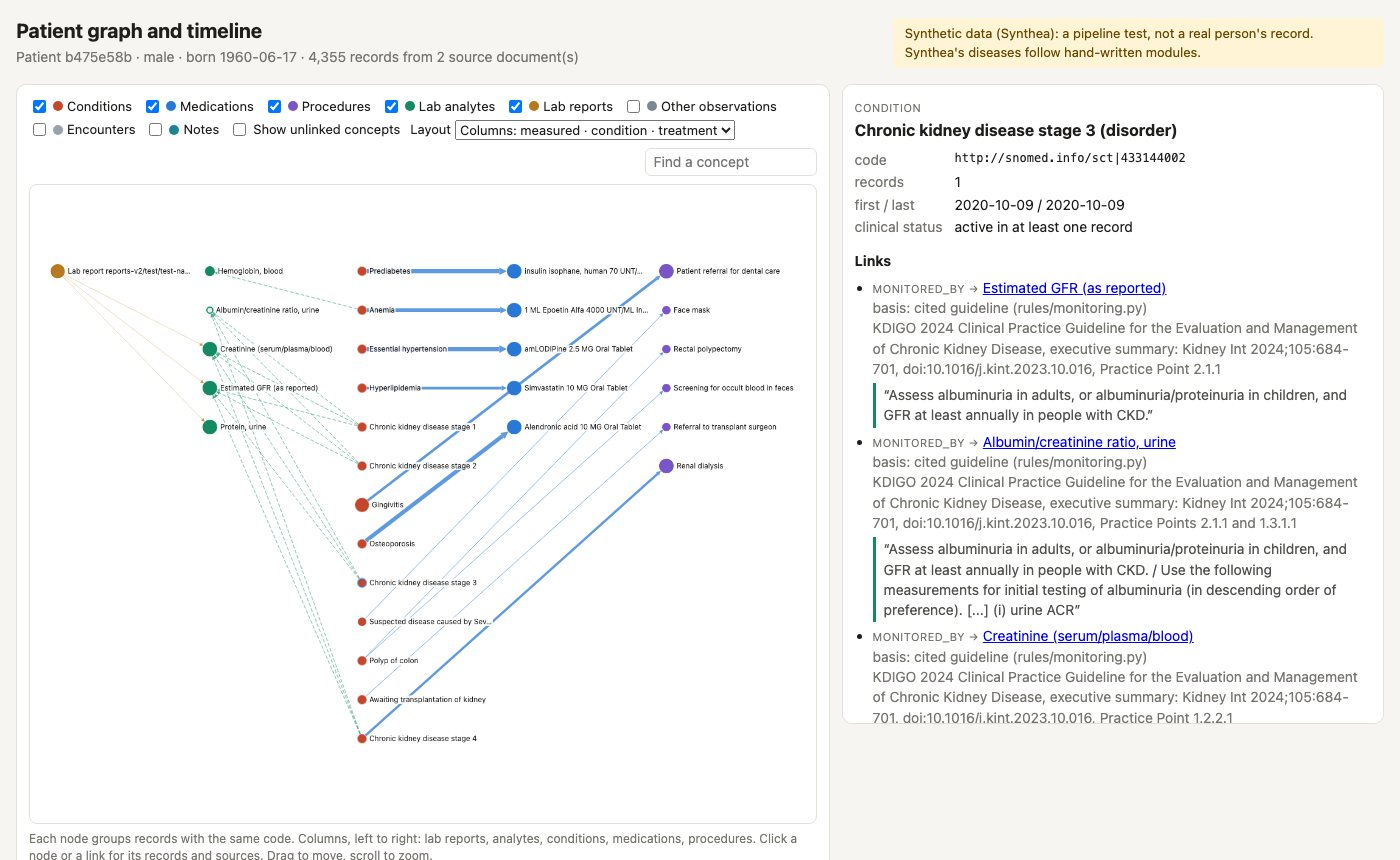
\includegraphics[width=\linewidth]{figures/viewer-patient.jpg}
\caption{The viewer on a synthetic patient with CKD, anaemia and one filed lab report. The CKD stage~3 concept is selected; the side panel shows its guideline links with source and verbatim quote. The timeline is below the fold.}
\label{fig:viewer}
\end{figure}

\subsection{Cohort build and invariants}
\code{scripts/build_graphs.py} builds every patient and checks the invariants in \code{graph/check.py}:
\begin{itemize}[nosep]
  \item every node has valid attributes and a source (analyte concepts excepted);
  \item every edge joins the kinds its type allows, and every guideline edge carries a citation and a quote;
  \item every usable lab result is in exactly one series;
  \item every usable report row is in a series or repeats a value that is;
  \item no unusable value is in a series;
  \item the \code{precedes} edges match the series order;
  \item every record and report row has its node.
\end{itemize}
The 156 synthetic reports of reports-v1 and reports-v2 are filed in the record of the patient whose tag they print. Their transcriptions are read from the saved LLM runs (no model is called), checked against the text hash and prompt version, and interpreted again with the current code.

\begin{table}[h]
\centering\small
\begin{tabularx}{\linewidth}{@{}>{\raggedright\arraybackslash}X r@{}}
\toprule
dev-1000 (synthetic) & \\
\midrule
patients built / invariant violations / build issues & 1,148 / \textbf{0} / 0 \\
nodes / edges & 977,475 / 1,152,231 \\
nodes per patient (min / median / max) & 27 / 384 / 18,855 \\
medication requests naming a reason (\code{treated_by}) & 41,953 of 54,181 (77\%) \\
procedures naming a reason & 38,466 of 144,713 (27\%) \\
condition records with guideline links: CKD 1--4 / anaemia & 266 / 383 \\
reports filed; report rows (ok / unmapped / eGFR in mL/min / misplaced) & 156; 279 / 915 / 13 / 2 \\
reports without a collection date (rows off the timeline) & 18 \\
\textbf{usable report rows repeating exactly one FHIR result} & \textbf{243 of 243} \\
\quad matching no FHIR result / more than one & 0 / 0 \\
store digest, rebuilt under a different string-hash seed & identical (\texttt{17bc4588\ldots}) \\
store size; build time (Apple M3) & 1.3\,GB; 8--10 min \\
\bottomrule
\end{tabularx}
\caption{The dev-1000 graphs (\code{docs/data/synthea-dev-1000-graphs.md}).}
\label{tab:graphs}
\end{table}

\paragraph{Reading the results.}
\begin{itemize}
  \item \textbf{243 of 243 is a check on extraction, from a different angle.} Every synthetic report was printed from FHIR values. A usable row matching nothing would be a wrong value or date that got through, or a failure of matching. None did, across reports-v1 and reports-v2.
  \item \textbf{The 18 undated reports} are exactly the 11 reports-v1 and 7 reports-v2 reports whose dates Phase~1e refused.
  \item \textbf{Values set aside are visible, not lost.} For example, 3,490 eGFR values recorded in mL/min (not normalized to body surface area) cannot be converted, and 46 creatinine values fall outside the sanity bounds. Both stay as nodes with their reason.
\end{itemize}

\subsection{Deviations from the approved plan}
\begin{itemize}[nosep]
  \item \textbf{Patient details} sit on the graph itself, not on a patient node: one graph holds one patient.
  \item \textbf{No separate \code{measured_at} edge.} Lab results use \code{occurred_during} like every other record.
  \item \textbf{Added} a \code{lab_report} node and a \code{part_of} edge, so a report's date, conventions and issues belong to the report.
  \item \textbf{Same measurement at the printed precision}, as described above, instead of equal canonical values.
  \item \textbf{DiagnosticReports are not nodes.} Their notes are note nodes citing both resources; lab-panel grouping is not in the graph yet.
\end{itemize}

%=====================================================================================
\section{Engineering log: problems found and fixed}
These problems would have produced wrong numbers, misleading provenance or a broken review if left alone.

\begin{table}[h]
\centering\footnotesize
\begin{tabularx}{\linewidth}{@{}>{\raggedright\arraybackslash}p{4.6cm}>{\raggedright\arraybackslash}X>{\raggedright\arraybackslash}p{4.0cm}@{}}
\toprule
Problem & Risk & Fix \\
\midrule
A date with equal fields counted as proof of day-first & Two en-US collection dates swapped & Equal fields prove nothing; caught by the new ``date wrong'' metric; pinned by a test \\
A concept link in the viewer showed the basis of its first record edge & One record's provenance shown for many & Concept links state a basis true of every edge they group \\
The store closed its connection inside a transaction on a schema mismatch & Crash instead of a clear refusal & Version checked after the transaction; tested \\
The side panel rendered ``[object HTMLTableElement]'' & Record lists unreadable & Children flattened fully; found by a headless-browser check \\
Graph labels hidden at the default zoom (dots only) & Graph unreadable without zooming & Column layout by kind; semantic tags dropped from labels \\
\code{.gitignore}'s \code{data/} also matched \code{docs/data/} & The aggregate data reports had never been committed & Patterns anchored to the repository root \\
The review notebook used a pandas feature that needs jinja2, absent from the kernel's environment & Notebook failed for the user although \code{make review} passed & \code{make review} now runs in the kernel's own environment \\
Report figures embedded their creation date & Regenerated figures never byte-identical & Creation date omitted; reruns reproduce the bytes \\
\bottomrule
\end{tabularx}
\caption{Problems found during Phases 1e and 2.}
\end{table}

%=====================================================================================
\section{Limitations and threats to validity}
\begin{enumerate}
  \item \textbf{Synthetic data throughout.} Synthea fills \code{reasonReference} and codes conditions from its own modules. Real records often leave reasons empty, and then \code{treated_by} is missing. A missing link is never inferred, and it is not evidence of an untreated condition.
  \item \textbf{The row-order check assumes name, value, unit, range.} A value-first or range-first layout would lose its rows: recall is lost, but no wrong value gets through. Its catch rate rests on two rows and the unit tests.
  \item \textbf{Clock times are skipped only after a time word.} A bare \texttt{08.30} in an Italian report counts as proof of a decimal point. If the report also contains a decimal comma, the contradiction surfaces as an issue rather than a wrong value; otherwise it goes unseen.
  \item \textbf{Exact code matching.} Without a SNOMED CT hierarchy, a more specific anaemia code gets no guideline link until it is listed.
  \item \textbf{Two different measurements can merge.} Two measurements with the same analyte, day and value at the printed precision count as one. No value changes, but same-day repeats can be undercounted.
  \item \textbf{The same report filed twice} as two files (text and PDF) would give two report nodes. Report-only rows would then appear twice. Detecting duplicate documents belongs to Phase~5.
  \item \textbf{Filing by the printed patient tag} is a test harness for synthetic reports. In the application, a person files a report into a record.
  \item \textbf{The viewer is English only}, and a value known only by its date is drawn at noon UTC.
\end{enumerate}

%=====================================================================================
\section{Next: Phase 3}
Phase~3 adds guideline rules and follow-up flags for CKD and anaemia. The user decided three points:
\begin{itemize}[nosep]
  \item \textbf{CKD persistence is strict:} two abnormal values at least 90 days apart, with no normal value between.
  \item \textbf{For anaemia, the most recent usable haemoglobin decides.}
  \item \textbf{Medication-monitoring flags move to Phase~4,} together with the drug labels they must cite.
\end{itemize}

The other inputs:
\begin{itemize}[nosep]
  \item \textbf{eGFR:} computed with CKD-EPI 2021 (Inker et al., N Engl J Med 2021;385:1737--49) from creatinine, age and administrative gender (used as a proxy for sex, and stated as such). It is shown as its own series, never mixed with reported eGFR.
  \item \textbf{Anaemia cutoffs:} WHO 2024, verified against the primary text before coding.
  \item \textbf{What every flag carries:} its evidence (values, dates, sources), its citations, its limitations and its rule version.
\end{itemize}
Agreement with Synthea's own diagnosis codes will be reported as a consistency check only. Synthea codes its conditions from its own models, so agreement is not accuracy, and the rules are never tuned to match it.

\appendix
%=====================================================================================
\section{Reproducing the results}
From the repository root, with \code{MEDGRAPH_DATA_DIR} pointing at the data drive:
\begin{Verbatim}
make check                          # ruff, mypy --strict, pytest (426 tests + 2 opt-in)
uv run python scripts/generate_lab_reports.py configs/lab_reports/reports-v2.yaml
make extract-rules SPLIT=test RULES=rules-r2
make extract-llm SPLIT=test LLM=qwen35-9b-r2 OLLAMA_MODELS=/Volumes/T7/ollama-models  # ~3 h
make graphs                         # every dev-1000 graph, checked and stored (~10 min)
make view PATIENT=b475e58b          # one patient's offline page
make report                         # figures from saved metrics, then both PDFs
make review                         # re-run notebooks/review.ipynb
\end{Verbatim}
Decisions: \code{docs/decisions/0004} (Phase 1e) and \code{0005} (Phase 2). Results: \code{docs/results/*-r2-test.md} and \code{docs/data/synthea-dev-1000-graphs.md}.

\section{Code and tests}
The library now has 3,811 lines of Python in \code{src/medgraph}, plus 843 lines of viewer HTML, CSS and JavaScript. The scripts have 3,484 lines and the tests 3,099. Of 428 tests, 426 run by default; two opt-in tests need the generated cohort. New in these phases:
\begin{itemize}[nosep]
  \item the row-order check, with five positive and five negative cases;
  \item separator and date-order evidence, including equal fields;
  \item every edge kind, determinism under two string-hash seeds, and the printed-precision rule at its boundaries;
  \item the SQLite round trip, foreign keys and tamper detection, and one test per invariant showing it catches its corruption;
  \item the viewer: pinned hashes, no network loads, safe embedding of hostile record text, and a static guard against HTML injection in the page script;
  \item an opt-in test that builds, checks and round-trips every 50th dev-1000 patient.
\end{itemize}

\end{document}
